\documentclass[titlepage]{jarticle}
\usepackage{h31ec-exp}
\usepackage[dvipdfmx]{graphicx}
\usepackage{here}

\title{RとCの回路の充放電特性}
\grade{2年40番}%
\author{鷲尾 優作}
\team{}
\date{令和2年7月6日}
\expdate{令和2年7月1日}
\coauthor{%
  26番 & 滝沢 倖大\\
  31番 & 原山 蓮\\
  34番 & 西脇 光}

\begin{document}
\maketitle

\section{本実験の目的}
\begin{itemize}
    \item 電気回路において,電圧を加えた瞬間や切った瞬間に起こる定常とは異なる動作(過渡現象)といい,有害なこともあるが電子回路ではこの特性を利用することも多い
    \item 直流の場合のRとCの直列回路の充電,放電特性を測定することを通して,RC回路に生ずる過渡現象とその時定数を知る
\end{itemize}

\section{理論}
コンデンサに電流が流れ込むと電荷が蓄えられる.コンデンサの端子間電圧を測定することでこの様子を間接的に見ることができる.
電荷が蓄えられていないときは0[V],少しでも蓄えられていればいくらかの電圧を測定できる.\\
\begin{figure}[H]
    \begin{center}
        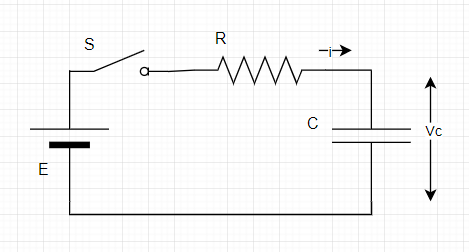
\includegraphics[width=10cm]{image/1.png}
        \caption{コンデンサの充電}
    \end{center}
\end{figure}

図1の充電を考える.Sをオンにし電圧を加えると,Cに電流が流れ充電が始まる.時間が十分経過してコンデンサの電圧$V_C$が電源の電圧Cと等しくなると,充電が終わり電流が流れなくなる.\\

\begin{figure}[H]
    \begin{center}
        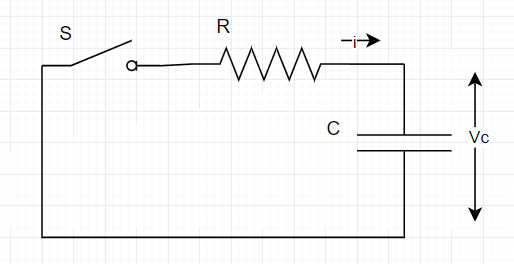
\includegraphics[width=10cm]{image/2.png}
        \caption{コンデンサの放電}
    \end{center}
\end{figure}
図2は電圧としてE=($V_C$)充電されたコンデンサの放電の様子を示している.$V_C$が0[V]になると,放電が終わり電流が流れなくなる.\\

「コンデンサは直流を流さない」と表現することがある.\\
これは電圧を加えてから十分時間が経過した(定常状態),充電や放電が終わった後でのことである.ここでの例のように,電圧を加えた瞬間は定常状態とは異なる動作となる.充電放電が速ければ,早くに定常状態となりうる.

充放電の速さは$R * C$[s]で決まる$R * C$を時定数といい,t(タウ)で表す.RC回路の充放電において,時間が時定数τ経過後のコンデンサの電圧は,最終値の63.2\%の値に達する.\\
RやCがそれぞれ異なっている回路でもτが等しければ,同様な動作をする.

\section{実験内容}
図4はRC回路の充放電特性を測定する回路である.RとCはブレッドボード上で接続する.\\
スイッチSは中心位置ではどこにも接続されない.また,Sは充電特性を測定するときにはグランド側,放電特性を測定するときには直流電源側に接続されるようにする.
\begin{figure}[H]
    \begin{center}
        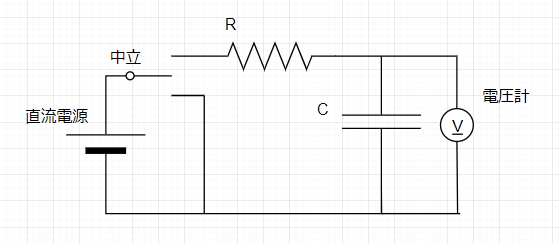
\includegraphics[width=10cm]{image/3.png}
        \caption{コンデンサの充放電特性}
    \end{center}
\end{figure}


\section{使用器具}
\begin{enumerate}
    \item 直流電源装置\\用途 直流電源確保のため\\商品名KIKUTU PMC18-3\\定格 INPUT AC100V 50/60Hz Max 230VA\\物品番号Ec-09
    \item 抵抗器\\用途 測定対象として使用するため\\商品名不明\\炭素皮膜抵抗器 47[kΩ]1本 22[kΩ]1本 68[kΩ]1本 33[kΩ]1本\\物品番号なし
    \item コンデンサ\\用途 測定対象として使用するため\\商品名不明\\電解コンデンサ 1000[µF]1本 2200[µF]1本\\物品番号なし
    \item 電圧計\\用途 実験データ計測のため\\商品名YOKOGAWA MODEL2011 CLASS0.5 B9000EU\\定格 0-100V 1000Ω/V\\物品番号不明
\end{enumerate}

\section{測定}
RC回路充放電特性の測定結果として図5のような結果が欲しい.充放電特性の測定,放電特性の測定の順で行う.
\subsection{充電特性}
\begin{enumerate}
    \item R=47[kΩ],C=1000[μF]で回路を組み接続する.
    \item 直流電源の電圧E=10[V]に設定する
    \item スイッチSをグランド側に接続されるよう設定し,コンデンサの電圧が0[V]になっていることを確認する.
    \item スイッチSを直流電源側に接続されるように設定すると同時にストップウォッチをスタートさせる.
    \item コンデンサの電圧が1,2,...,9,10[V]になったときの時間を測定し表1のようにまとめる.
    \item RCの組み合わせを次のように変えて,測定を繰り返す\\R=22[kΩ],C=2200[μF] R=68[kΩ],C=1000[μF] R=33[kΩ],C=2200[μF]
\end{enumerate}
\subsection{放電特性}
\begin{enumerate}
    \item R=47[kΩ],C=1000[μF]で回路を組み接続する.
    \item 直流電源の電圧E=10[V]に設定する
    \item スイッチSを直流電源側に接続されるよう設定し,コンデンサの電圧が10[V]になっていることを確認する.
    \item スイッチSをグランド側に接続されるように設定すると同時にストップウォッチをスタートさせる.
    \item コンデンサの電圧が10,9,...,2,1,0[V]になったときの時間を測定し表2のようにまとめる.
    \item RCの組み合わせを次のように変えて,測定を繰り返す\\R=22[kΩ],C=2200[μF] R=68[kΩ],C=1000[μF] R=33[kΩ],C=2200[μF]
\end{enumerate}

\section{測定結果}
\subsection{測定方法}

\begin{table}[htbp]
    \caption{}
    \begin{tabular}{c|c|c|c|c}
        \multicolumn{ 5}{c}{RC回路の充電特性}                                                       \\ \hline
                & R=47[kΩ]C=1000[μF] & R=22[kΩ]C=2200[μF] & R=68[kΩ]C=1000[μF] & R=33[kΩ]C=2200[μF] \\ \hline
        電圧[V] & 計測値[s]          & 計測値[s]          & 計測値[s]          & 計測値[s]          \\ \hline\hline
        0       & 0.0                & 0.0                & 0.0                & 0.0                \\ \hline
        1       & 5.3                & 5.5                & 3.7                & 7.9                \\ \hline
        2       & 10.8               & 11.1               & 11.8               & 16.7               \\ \hline
        3       & 17.3               & 17.8               & 20.9               & 26.9               \\ \hline
        4       & 24.9               & 25.4               & 31.7               & 38.8               \\ \hline
        5       & 34.3               & 35.9               & 43.9               & 52.9               \\ \hline
        6       & 45.9               & 46.1               & 59.3               & 69.9               \\ \hline
        7       & 64.1               & 60.6               & 78.9               & 92.7               \\ \hline
        8       & 86.6               & 81.7               & 105.8              & 125.0              \\ \hline
        9       & 124.0              & 117.7              & 150.0              & 181.4              \\ \hline
        10      & 239.8              & 222.6              & 243.9              & 286.9              \\ \hline
    \end{tabular}
    \label{}
\end{table}


\begin{table}[htbp]
    \caption{}
    \begin{tabular}{c|c|c|c|c}
        \multicolumn{ 5}{c}{RC回路の放電特性}                                                       \\ \hline
                & R=47[kΩ]C=1000[μF] & R=22[kΩ]C=2200[μF] & R=68[kΩ]C=1000[μF] & R=33[kΩ]C=2200[μF] \\ \hline
        電圧[V] & 計測値[s]          & 計測値[s]          & 計測値[s]          & 計測値[s]          \\ \hline\hline
        10      & 0.0                & 0.0                & 0.0                & 0.0                \\ \hline
        9       & 4.6                & 6.9                & 5.8                & 7.9                \\ \hline
        8       & 10.3               & 13.1               & 14.2               & 16.8               \\ \hline
        7       & 17.0               & 19.7               & 24.6               & 27.2               \\ \hline
        6       & 24.9               & 27.4               & 35.8               & 39.1               \\ \hline
        5       & 33.9               & 36.7               & 51.7               & 53.2               \\ \hline
        4       & 45.8               & 48.0               & 65.1               & 70.1               \\ \hline
        3       & 60.5               & 62.8               & 86.0               & 99.1               \\ \hline
        2       & 81.5               & 84.0               & 118.1              & 125.4              \\ \hline
        1       & 118.5              & 120.2              & 169.6              & 180.6              \\ \hline
        0       & 260.7              & 270.8              & 362.6              & 400.2              \\ \hline
    \end{tabular}
    \label{}
\end{table}


\subsection{測定結果}
\begin{figure}[H]
    \begin{center}
        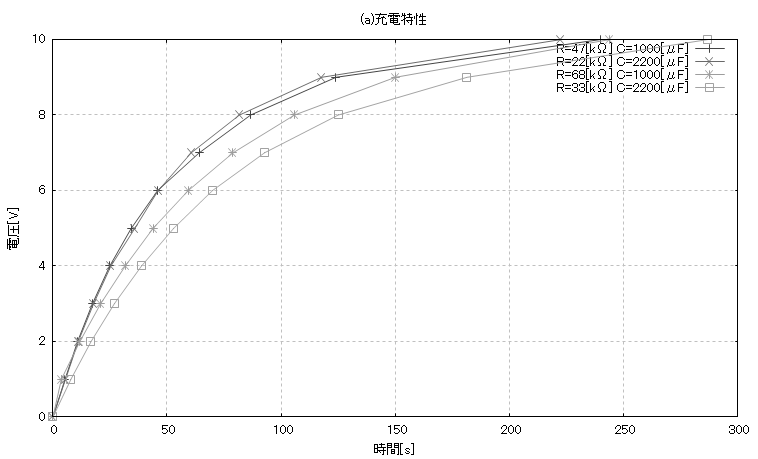
\includegraphics[width=15cm]{graph/1.PNG}
    \end{center}
\end{figure}

\begin{figure}[H]
    \begin{center}
        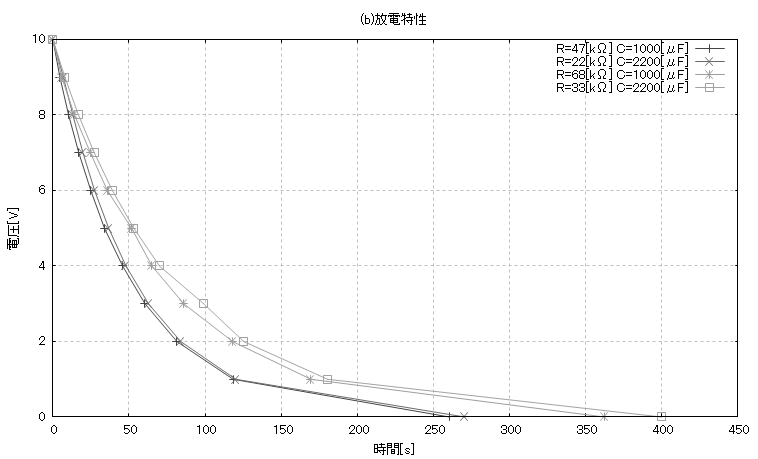
\includegraphics[width=15cm]{graph/2.PNG}
        \caption{RC回路の特性}
    \end{center}
\end{figure}

\section{課題考察}
\begin{enumerate}
    \item 時定数は理論値と一致したか,一致しないとすればどのような原因が考えられるか.\\その対策はどうすればよいか.\\
          時定数はそれぞれ\\
          R=47[kΩ]C=1000[μF]の場合\\
          理論値は$τ=R*C=47[kΩ]*1000[μF]=47[s]$\\
          実測値は,53.5[s]\\\\
          R=22[kΩ]C=2200[μF]の場合\\
          理論値は$τ=R*C=22[kΩ]*2200[μF]=48.4[s]$\\
          実測値は,51.9[s]\\\\
          R=68[kΩ]C=1000[μF]の場合\\
          理論値は$τ=R*C=68[kΩ]*1100[μF]=68[s]$\\
          実測値は,67.2[s]\\\\
          R=33[kΩ]C=2200[μF]の場合\\
          理論値は$τ=R*C=33[kΩ]*2200[μF]=72.6[s]$\\
          実測値は,115.0[s]\\\\
          となりおおむね一致しているが,誤差とは言い難い差が出ているものもあった。対策としては計測時間の精度を上げること,RCのそれぞれの定数をあらかじめ実測することが考えられる.
    \item 時定数の大小によって特性曲線はどう変わるか\\
          時定数は、定常状態の63.2[\%]に達するまでの時間といえるので,時定数が大きくなるほど、グラフはx軸方向に引き延ばされた形になる.
\end{enumerate}


\section{感想}
手で計測できるモノなのかと感じたが,RCの定数がうまく調整されていてストップウォッチでかなり精度よく計測でき,
実際に回路内で使用する際,確かに不便であり,便利そうだと確認できた.\\
時定数の計算,意味をもう少し時間をかけて理解したい.

\end{document}